%!TEX TS-program = xelatex
\documentclass[a4paper, 12pt]{article}
\usepackage{barinovxesimple}
\geometry{top=25mm}
\geometry{bottom=35mm}
\geometry{left=35mm}
\geometry{right=20mm}
\setlist{labelindent=\parindent,leftmargin=*}
\begin{document}
\thispagestyle{empty}
\begin{center}
    \textit{Федеральное государственное автономное образовательное\\ учреждение высшего образования }

    \vspace{0.5ex}

        \textbf{«Московский физико-технический институт\\ (национальный исследовательский университет)»}
\end{center}

\vspace{10ex}

\begin{center}
    \vspace{13ex}

    \so{\textbf{Лабораторная работа №-.-.-}}

    \vspace{1ex}

    по курсу общей физики

    на тему:

    \textbf{\textit{<<>>}}

    \vspace{30ex}

    \begin{flushright}
        \noindent
        \textit{Работу выполнил:}\\  
        \textit{Баринов Леонид \\(группа Б02-827)}
    \end{flushright}
    \vfill
    Долгопрудный \\2019
\newpage
\setcounter{page}{1}
\fancyhead[R]{\nouppercase{\leftmark}}	
\end{center}

\section{Цель работы}
В работе исследуются сериальные закономерности в оптическом спектре
водорода и спектр поглощения паров йода в видимой области.

\section{Суть исследуемого явления}

Спектр атома --- набор частот, испускаемых возбужденным атомом.
Экспериментально спектр определяется с хорошей точностью, поэтому
представляет интерес сравнить эти экспериментальные данные с теорией.

Особенно хорошо получается провести процесс сравнения теории явления и
наблюдаемого спектра на атоме водорода и водородноподобных
(одноэлектронных) атомах, для которых уравнение Шредингера \eqref{eq:2}  может быть
решено точно.

\section{Теория явления}
Одним из основных утверждений квантовой механики является утверждение,
что состояние, в котором физическая величина $f$ имеет определенное
значение $f_0$, описывается $\psi$-функцией, являющейся решением
уравнения:
\begin{equation}
    \hat f \psi = f_0 \psi 
    \label{eq:1}
\end{equation}

У изолированных систем сохраняется энергия, следовательно их состояния
описываются $\psi$-функциями. Подставляя в \eqref{eq:1} вместо $\hat
f$ оператор полной энергии, получим уравнение Шредингера для
стационарных состояний:
\begin{equation}
    - \frac{\hbar^2}{2m} \Delta \psi + U \psi = E_0 \psi
    \label{eq:2}
\end{equation}
$U$ --- потенциальная энергия. В случае водородноподобного атома она
будет выражаться кулоновским взаимодействием ядра и электрона:
\begin{equation}
    U (r) = - \frac{Z e^2}{r}
    \label{eq:3}
\end{equation}
где $Z$ --- заряд ядра.

Уравнение Шредингера \eqref{eq:2} с потенциальной энергией
\eqref{eq:3} может быть решено точно. Энергетические состояния будут
определяться выражением:
\begin{equation}
    E_n = - \frac{2 \pi^2 m_e e^4 Z^2}{h^2} \frac{1}{n^2}
    \label{eq:4}
\end{equation}

В формуле \eqref{eq:4} выделяют постоянную Ридберга:
\begin{equation}
    R = \frac{2 \pi^2 m_e e^4}{h^3 c}
    \label{eq:5}
\end{equation}

Излучение или поглощение происходит при
переходе электрона с одной орбиты на другую, при этом частота
излучения
\begin{equation}
    h\nu = E_1 - E_2
    \label{eq:6}
\end{equation}


\begin{wrapfigure}{l}{0.4\linewidth}
    \includegraphics[width=\linewidth]{1}
    \caption{Уровни энергии атома водорода и образование спектральных
    серий}
    \label{fig:1}
\end{wrapfigure}

Тогда при переходе электрона в атоме водорода с уровня $m$ на уровень
$n$ 
длина волны излучения: 
\begin{equation}
    \frac{1}{\lambda} = R \left( \frac{1}{n^2} - \frac{1}{m^2} \right)
    \label{eq:7}
\end{equation}

Из \fig{fig:1} видно, что линии в спектре водорода можно расположить
по сериям; для всех линий серии значение $n$ остается постоянными, а
$m$ может принимать любые значения от $n+1$ до $\infty$. В данной
работе изучается серия Бальмера, линии которой лежат в видимой
области. Для серии Бальмера $n=2$. Величина $m$ для первых четырех
линий этой серии принимает значение $3, 4, 5, 6$. Это линии обозначаются
символами $H_\alpha, H_\beta, H_\gamma, H_\delta$.

Молекулы обладают более богатым спектром возбужденных состояний, так
как обладают колебательными и вращательными подуровнями. В первом
приближении $E = E_\text{эл} + E_\text{кол} + E_\text{вращ}$. Энергия
колебательных состояний примерно в $10^3$ меньше энергии электронных
переходов $E_\text{эл}$, энергия вращательных состояний
$E_\text{вращ}$ меньше $E_\text{эл}$ примерно в $10^6$ раз, в связи с
чем обнаружить $E_\text{вращ}$ спектроскопическим методом в данной
работе невозможно.


\begin{figure}[H]
    \includegraphics[width=0.6\linewidth]{2} 
    \caption{Электронные и электронно-колебательные энергетические
    уровни двухатомной молекулы}
    \label{fig:2}
\end{figure}

На \fig{fig:2} схематически изображены энергетические уровни молекулы
без учета вращательной структуры. Штриховыми линиями показаны чисто
электронные уровни $E_1$ и $E_2$, а сплошными --- колебательные
подуровни этих состояний. Минимальное значение колебательной энергии
при $n = 0$ отлично от нуля и равно $h \nu / 2$. C ростом квантовых
чисел $n_1$ и $n_2$ колебательные подуровни сближаются и переходят в
непрерывный спектр, области которого на рисунке заштрихованы. С ростом
$n$ растет амплитуда колебаний, при достижении некоторой максимальной
амплитуды происходит разрыв связи между атомами --- диссоциация
молекулы.

Наименьшая энергия, которую нужно сообщить молекулы в нижайшем
колебательном состоянии $(n  = 0)$, чтобы она диссоциировала,
называется энергией диссоциации. На \fig{fig:2} $D_1$, $D_2$ ---
энергия диссоциации молекулы из состояний $n_1 = 0$ и $n_2 = 0$; $E_a$
--- энергия возбуждения атома, возникающая при переходе молекулы из
состояния 1 в область непрерывного спектра, соответствующего состоянию
2; $h\nu_\text{эл}$ --- энергия чисто электронного перехода; $h
\nu_\text{гр}$ --- энергия возбуждения, при которой происходит переход
молекулы в область непрерывного спектра.

Спектр поглощения йода в видимой области при комнатной температуре
состоит из двух серий Деландра (нулевая и первая).


\begin{figure}[H]
    \floatsetup{heightadjust=object,valign=c}
    \begin{floatrow}

        \ffigbox{
        \caption{Структура электронно-колебательного спектра
        поглощения молекулы йода в видимой области}
    }
        {
        \includegraphics[width=\linewidth]{3}
    }

        \ffigbox{
        \caption{Спектр поглощения паров йода}
    }
        {
        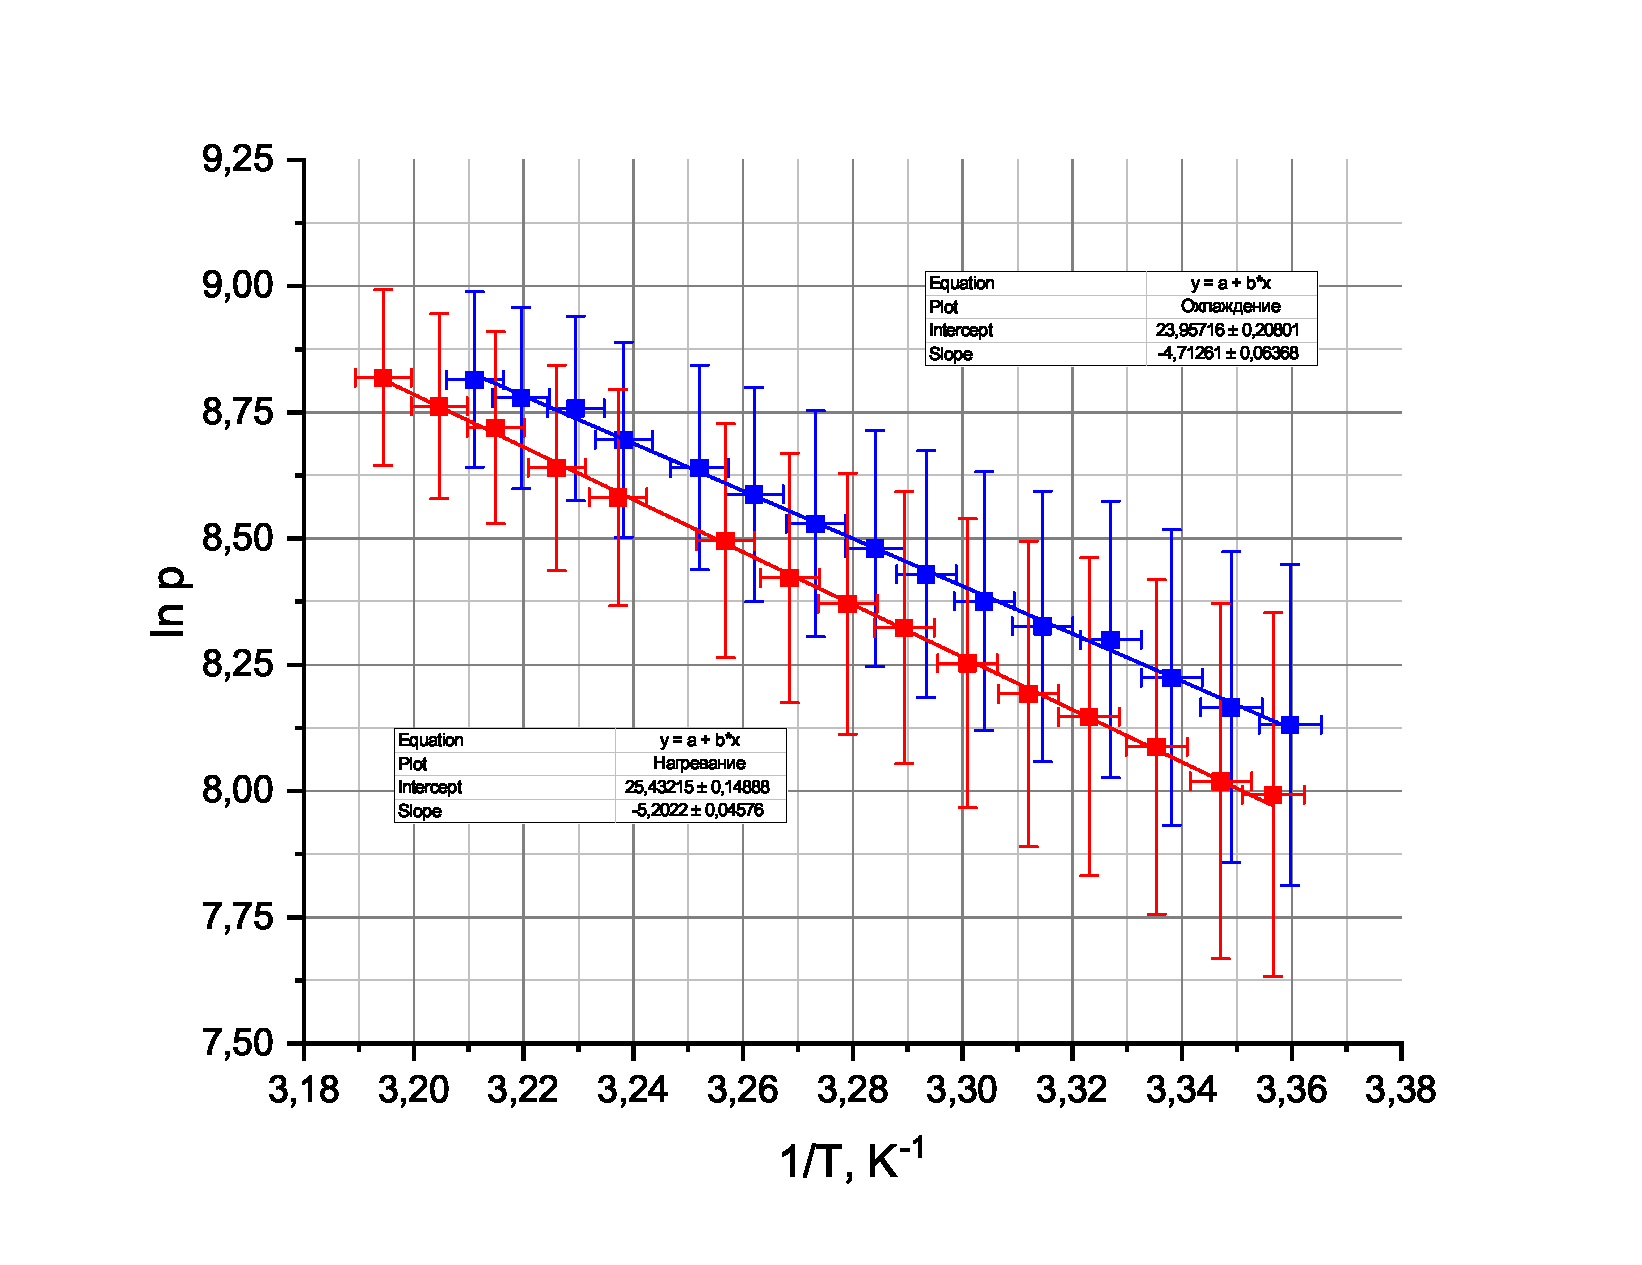
\includegraphics[width=0.9\linewidth]{4}
    }
    \end{floatrow}
\end{figure}

Энергетическое положение линий поглощения описывается выражением 
\begin{equation}
    h\nu_{0, n_2} = (E_2 - E_1) + h\nu_2 \left( n_2 + \frac{1}{2}
    \right) - \frac{1}{2}h\nu_1
    \label{eq:eq}
\end{equation}



\section{Эксперимент}


\subsection{Экспериментальная установка}


Для измерения длин волн спектральных линий в работе используется
стеклянно-призменный монохроматор-спектрометр УМ-2 (универсальный
монохроматор), предназначенный для спектральных исследований в
диапазоне от $0,38$ до $1,00\: \text{мкм}$.


Основные элементы монохроматора представлены на \fig{fig:5}. 1 ---
входная щель; 2 --- коллиматорный объектив; 3 --- спектральная призма;
4 --- объектив; 5 --- окуляр; 6 --- поворотный столик; 7 --- отсчетный
барабан; 8, 9 --- микрометрические винты; 10 --- острие указателя; 11
--- массивный корпус; \textsl{П}$_{1}$, \textsl{П}$_{2}$,
\textsl{П}$_{3}$ --- призмы; \textsl{Л} --- источник света;
\textsl{К} --- конденсатор.

В опытах по измерению длин волн балмеровской серии источником света
служит водородная трубка H-образной формы, питаемая от источника
высокого напряжения. В спектре водородной лампы наряду с линиями
атомного спектра наблюдается также спектр молекулярного водорода,
однако их интенсивность значительно слабее.


\begin{figure}[H]
    \floatsetup{heightadjust=object,valign=c}
    \begin{floatrow}

        \ffigbox{
        \caption{Схема экспериментальной установки для изучения
        спектра атома водорода}
    }
        {
        \includegraphics[width=\linewidth]{5}
        \label{fig:5}
    }

        \ffigbox{
        \caption{Схема экспериментальной установки для изучения
        молекулярного спектра йода}
    }
        {
        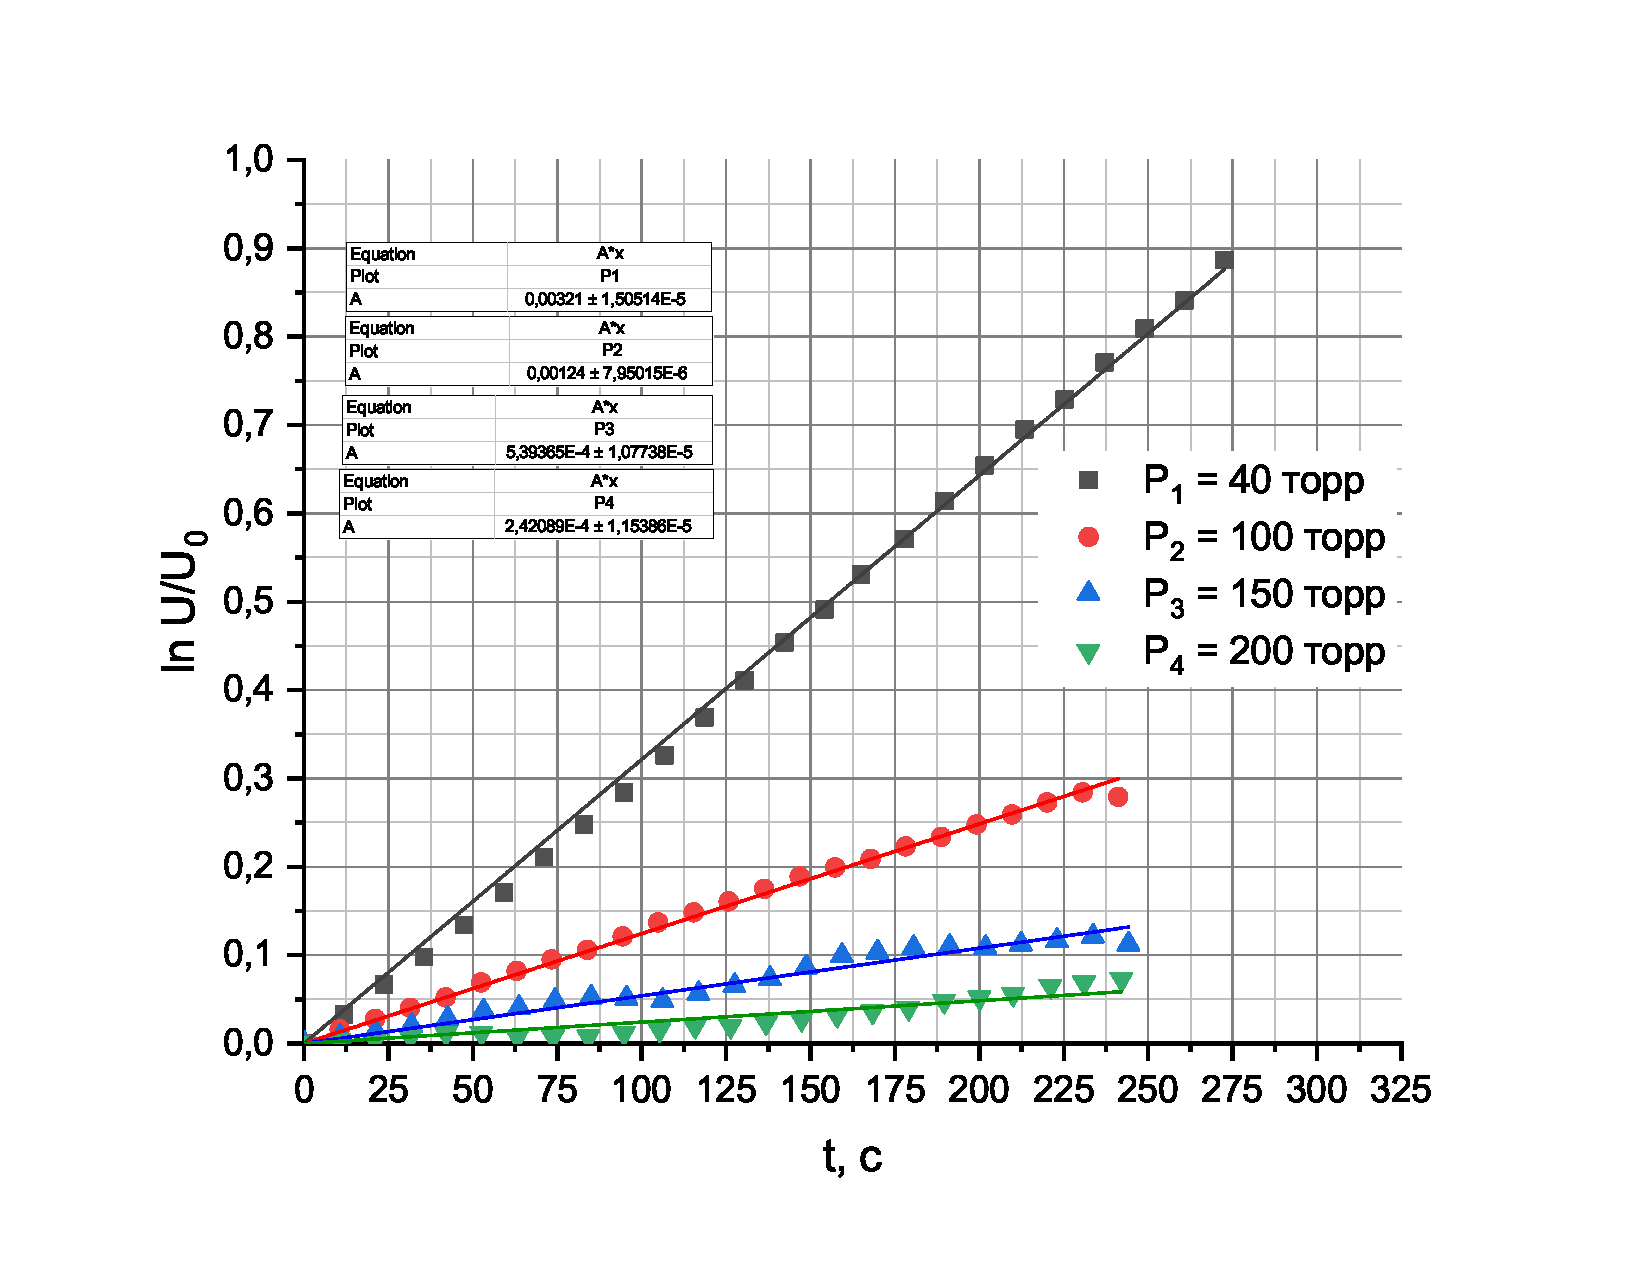
\includegraphics[width=\linewidth]{6}
        \label{fig:6}
    }
    \end{floatrow}
\end{figure}

На \fig{fig:6} изображена схема экспериментальной установки для
изучения молекулярного для изучения молекулярного спектра йода. 1
--- лампа накаливания; 2 --- блок питания; 3 --- кювета; 4 --- линза.

В нашей работе спектр поглощения паров йода наблюдается визуально на
фоне сплошного спектра лампы накаливания 1, питаемой от блока питания
2. Кювета 3 с кристаллами йода подогревается нихромовой спиралью,
подключённой вместе с лампой накаливания к блоку питания. Линза 4
используется как конденсор. В результате подогрева кристаллы йода
частично возгоняются, образуя пары с лёгкой фиолетовой окраской.
Спектрометр позволяет визуально наблюдать линии поглощения молекул
йода на фоне сплошного спектра излучения лампы накаливания видимой
области.


\section{Результаты эксперимента}
Калибруем барабан монохроматора с помощью спектров неона и ртути.

\renewcommand{\arraystretch}{1.5}
\begin{longtable}{|c|c|c|cccccc}
	\hline
        \multicolumn{6}{|c|}{$N\! e$} &
        \multicolumn{3}{c|}{$H\! g$}\\ \hline 
        №  & $\lambda, \: \mathring{A}$    & $\theta, ^{\circ}$   &
        \multicolumn{1}{c|}{№}  & \multicolumn{1}{c|}{$\lambda, \:
        \mathring{A}$}    & \multicolumn{1}{c|}{$\theta, ^{\circ}$}
        & \multicolumn{1}{c|}{№}  & \multicolumn{1}{c|}{$\lambda, \: \mathring{A}$}    & \multicolumn{1}{c|}{$\theta, ^{\circ}$}   \\ \hline
	\endfirsthead
	\hline
        \multicolumn{6}{|c|}{$N\! e$} &
        \multicolumn{3}{c|}{$H\! g$} \\ \hline 
        №  & $\lambda, \: \mathring{A}$    & $\theta, ^{\circ}$   &
        \multicolumn{1}{c|}{№}  & \multicolumn{1}{c|}{$\lambda, \:
        \mathring{A}$}    & \multicolumn{1}{c|}{$\theta, ^{\circ}$}
        & \multicolumn{1}{c|}{№}  & \multicolumn{1}{c|}{$\lambda, \: \mathring{A}$}    & \multicolumn{1}{c|}{$\theta, ^{\circ}$}   \\ \hline
        \endhead
	\endfoot
	\endlastfoot
1  & 7032 & 2596 & \multicolumn{1}{c|}{14} & \multicolumn{1}{c|}{6164} & \multicolumn{1}{c|}{2292} & \multicolumn{1}{c|}{К1} & \multicolumn{1}{c|}{6907} & \multicolumn{1}{c|}{2562} \\ \hline
2  & 6929 & 2564 & \multicolumn{1}{c|}{15} & \multicolumn{1}{c|}{6143} & \multicolumn{1}{c|}{2282} & \multicolumn{1}{c|}{К2} & \multicolumn{1}{c|}{6234} & \multicolumn{1}{c|}{2320} \\ \hline
3  & 6717 & 2504 & \multicolumn{1}{c|}{16} & \multicolumn{1}{c|}{6096} & \multicolumn{1}{c|}{2264} & \multicolumn{1}{c|}{1}  & \multicolumn{1}{c|}{5792} & \multicolumn{1}{c|}{2115} \\ \hline
4  & 6678 & 2490 & \multicolumn{1}{c|}{17} & \multicolumn{1}{c|}{6074} & \multicolumn{1}{c|}{2254} & \multicolumn{1}{c|}{2}  & \multicolumn{1}{c|}{5770} & \multicolumn{1}{c|}{2104} \\ \hline
5  & 6599 & 2461 & \multicolumn{1}{c|}{18} & \multicolumn{1}{c|}{6030} & \multicolumn{1}{c|}{2232} & \multicolumn{1}{c|}{3}  & \multicolumn{1}{c|}{5461} & \multicolumn{1}{c|}{1923} \\ \hline
6  & 6533 & 2434 & \multicolumn{1}{c|}{19} & \multicolumn{1}{c|}{5976} & \multicolumn{1}{c|}{2210} & \multicolumn{1}{c|}{4}  & \multicolumn{1}{c|}{4916} & \multicolumn{1}{c|}{1494} \\ \hline
7  & 6507 & 2426 & \multicolumn{1}{c|}{20} & \multicolumn{1}{c|}{5945} & \multicolumn{1}{c|}{2196} & \multicolumn{1}{c|}{5}  & \multicolumn{1}{c|}{4358} & \multicolumn{1}{c|}{821}  \\ \hline
8  & 6402 & 2388 & \multicolumn{1}{c|}{21} & \multicolumn{1}{c|}{5882} & \multicolumn{1}{c|}{2166} & \multicolumn{1}{c|}{6}  & \multicolumn{1}{c|}{4047} & \multicolumn{1}{c|}{265}  \\ \hline
9  & 6383 & 2380 & \multicolumn{1}{c|}{22} & \multicolumn{1}{c|}{5852} & \multicolumn{1}{c|}{2152} & \multicolumn{3}{c}{\multirow{4}{*}{}}                                           \\ \cline{1-6}
10 & 6334 & 2364 & \multicolumn{1}{c|}{23} & \multicolumn{1}{c|}{5401} & \multicolumn{1}{c|}{1883} & \multicolumn{3}{c}{}                                                            \\ \cline{1-6}
11 & 6305 & 2354 & \multicolumn{1}{c|}{24} & \multicolumn{1}{c|}{5341} & \multicolumn{1}{c|}{1841} & \multicolumn{3}{c}{}                                                            \\ \cline{1-6}
12 & 6267 & 2336 & \multicolumn{1}{c|}{25} & \multicolumn{1}{c|}{5331} & \multicolumn{1}{c|}{1834} & \multicolumn{3}{c}{}                                                            \\ \cline{1-6}
13 & 6217 & 2314 & \multicolumn{6}{c}{}  \\
\cline{1-3}                                     
\caption{Калибровка барабана монохроматора по спектрам неона и ртути}
\end{longtable}

По результатам в таблице 1 построим калибровочный график \ffig{fig:7}.
Аппроксимируем по дисперсионной формуле Гартмана:
\[
    \lambda = \lambda_0 + \frac{C}{\theta - \theta_0}
\]
\begin{figure}[H]
    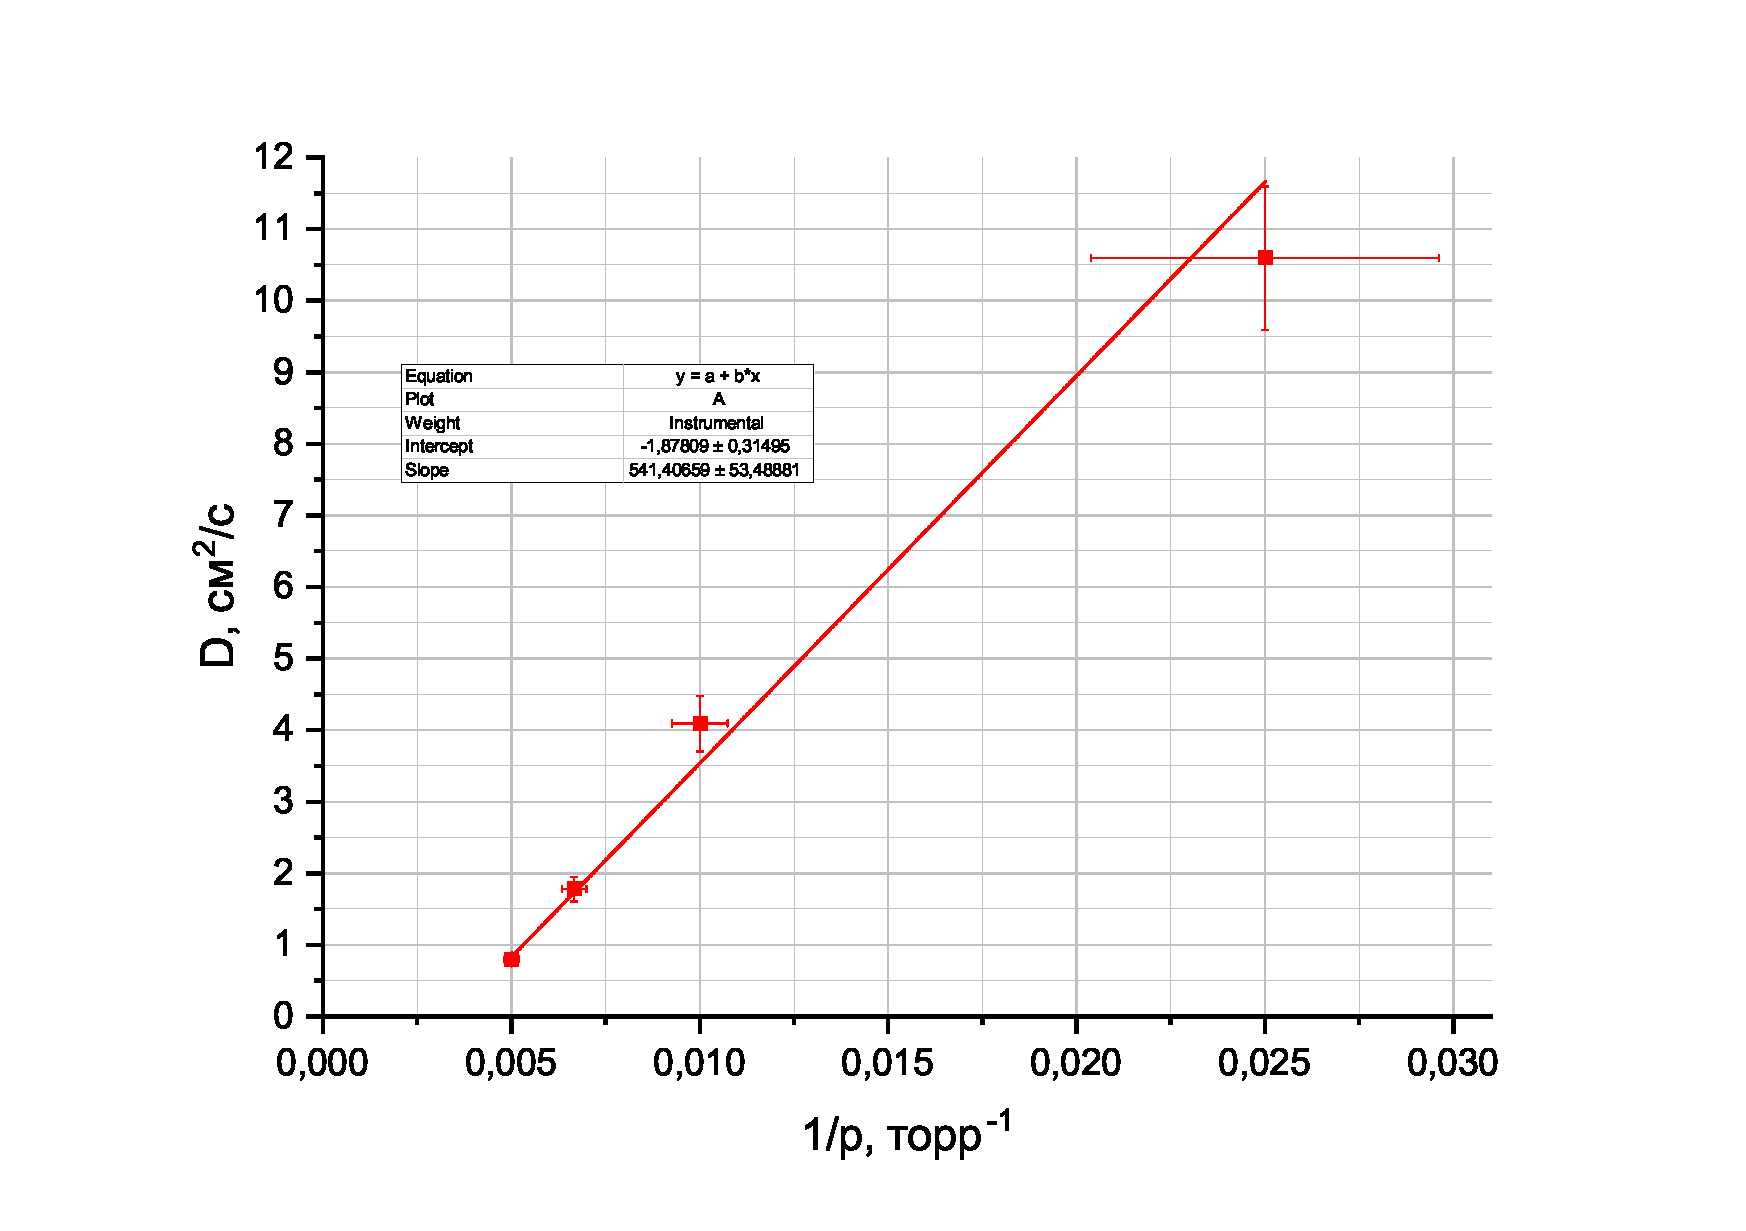
\includegraphics[width=0.90\linewidth]{7} 
    \caption{Калибровка барабана монохроматора по спектрам неона $N\!
    e$ и ртути $H\! g$}
    \label{fig:7}
\end{figure}

Рассмотрим линии спектра водорода и из градуировочной кривой определим
их длины волн. Результаты сведем в таблицу 2 и построим график связи
длины волны и номера перехода. 


\begin{table}[H]
\centering
\begin{tabular}{|c|c|c|c|c|c|}
\hline
Линия спектра & $\theta, \: ^{\circ}$  & $\lambda,\: \mathring{A}$  &
$m$ & $1/n^2-1/m^2$  & $1/\lambda,\: 10^{-4} \mathring{A}^{-1}$ \\ \hline
$H_\alpha$ & 2451 & 6571 & 3 & $0,139$ & $1,522$ \\ \hline
$H_\beta$ & 1464 & 4881 & 4 & $0,188$ & $2,049$ \\ \hline
$H_\gamma$ & 839 & 4368  & 5 & $0,210$ & $2,289$ \\ \hline
$H_\delta$ & 414 & 4123  & 6 & $0,222$ & $2,425$ \\ \hline
\end{tabular}
\caption{Определение линий спектра водорода}
\end{table}


\begin{figure}[H]
    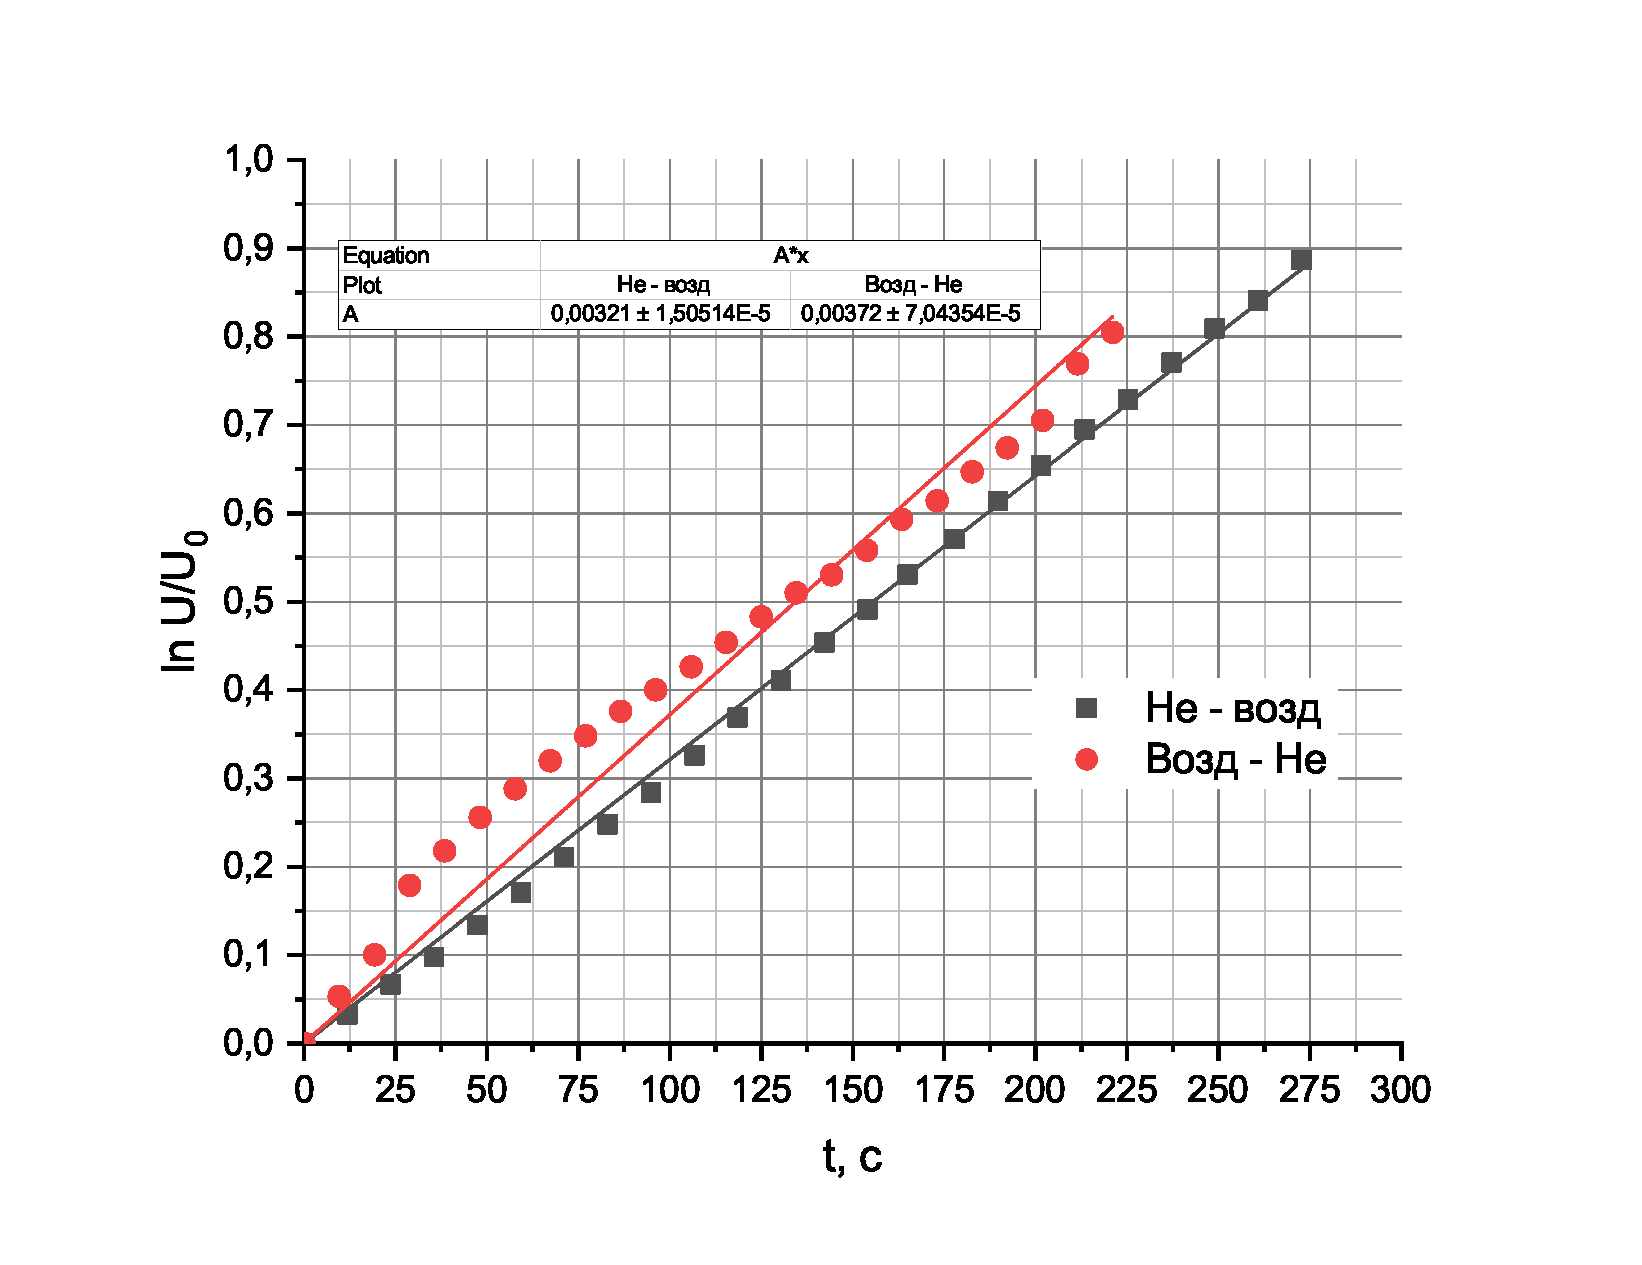
\includegraphics[width=0.9\linewidth]{8} 
    \caption{Проверка обобщенной формулы Бальмера \eqref{eq:7}}
    \label{fig:8}
\end{figure}





\section{Анализ результатов}

Из графика на \fig{fig:8} определим постоянную Ридберга:
\[
    R = (10,914 \pm 0,012) \cdot 10^{4}\: \text{см}^{-1}
\]

Исследуем спектр поглощения йода. Определим на монохроматоре деления,
соответствующие длинноволновой линии и линии, отстоящей на 6 от нее а
также границу схождения спектра.

\begin{equation*}
    \begin{gathered}
        \theta_{1, 0} = 2386 \Rightarrow \lambda_{1, 0} = 6394\:
        \mathring{A} \Rightarrow h\nu _{1, 0} \approx 1,94 \:
        \text{эВ}\\
        \theta_{1, 5} = 2282 \Rightarrow \lambda_{1, 5} = 6139\:
        \mathring{A} \Rightarrow h\nu _{1, 5} \approx 2,02 \:
        \text{эВ}\\
        \theta_{\text{гр}} = 1616 \Rightarrow \lambda_{\text{гр}} =
        5023\:
        \mathring{A} \Rightarrow h\nu _{\text{гр}} \approx 2,46 \:
        \text{эВ}
    \end{gathered}
\end{equation*}

Проведем расчеты энергии колебательного кванта возбужденного состояния
молекулы йода согласно \eqref{eq:eq}.
\[
    h\nu_2 = \frac{h\nu_{1, 5} - h\nu_{1, 0}}{5} = (0,0160 \pm 0,0007) \: \text{эВ} 
\]

Вычислим $h\nu_\text{эл} = E_2 - E_1$, сделав сдвиг серии на 1
(вычитая $h\nu_1 = 0,027\: \text{эВ}$):
\[
    h\nu_\text{эл} = h\nu_{1, 0} - \frac{1}{2}h\nu_2 + \frac{3}{2}h
    \nu_1 = (1,98 \pm 0,02) \: \text{эВ} 
\]

Получим энергии диссоциации частицы в основном $D_1$ и возбужденном
состоянии $D_2$, считая $E_a = 0,94\: \text{эВ}$.
\begin{equation*}
    \begin{gathered}
        D_1 = h\nu_\text{гр} - E_a = (1,52 \pm 0,03)\: \text{эВ}\\
        D_2 = h\nu_\text{гр} - h\nu_\text{эл} = (0,48 \pm 0,05)\:
        \text{эВ}
    \end{gathered}
\end{equation*}

\section{Выводы}
В работе было проведено исследование спектров водорода и йода в
видимой области. В спектре водорода в видимой области находится серия
Бальмера, в которой наблюдались первые четыре линии $H_\alpha,
H_\beta, H_\gamma, H_\delta$. С помощью калибровки монохроматора по
спектрам неона $N\! e$ и ртути $H\! g$ \ffig{fig:7} были определены длины волн
переходов четырех первых линий водорода при $n = 2$ (Таблица 2). По результатам
был построен график зависимости $1/\lambda$ от $1/n^2-1/m^2$
\ffig{fig:8}, который является линейным. Это является подтверждением
обобщенной формулы Бальмера \eqref{eq:7} и соответствует теории атома
Нильса Бора, также это позволяет вычислить
постоянную Ридберга:
\[
    R = (109140 \pm 120) \: \text{см}^{-1}
\]
Значение близкое к табличному:
\[
    R^\text{т} = 109678 \: \text{см}^{-1}
\]
Расхождения связаны с неточностью снятия спектра водорода.
Получившиеся значения $\lambda$ в таблице 2 отличаются от табличных
значений в среднем на $20\: \mathring{A}$.

В спектре йода в данной работе кроме электронных уровней наблюдаются
колебательные подуровни. Исходя из интенсивности спектра удалось
пронаблюдать 2 серии Деландра. По ним были проведены расчеты энергии
колебательного кванта возбужденного состояния молекулы йода, которая
получилась в 100 раз меньше энергии электронного перехода; вычислены
значения диссоциации частицы в основном $D_1$ и возбужденном состоянии
$D_2$:
\begin{equation*}
    \begin{gathered}
        D_1  = (1,52 \pm 0,03)\: \text{эВ}\\
        D_2  = (0,48 \pm 0,05)\:
        \text{эВ}
    \end{gathered}
\end{equation*}

Значение $D_1$ хорошо соотносится с табличным:
\begin{equation*}
        D_1 ^{\text{т}}  = 1,57\: \text{эВ}\\
\end{equation*}
Неточность полученных результатов связана с визуальным определением
линий спектра йода.



\end{document}
